%% LyX 2.0.3 created this file.  For more info, see http://www.lyx.org/.
%% Do not edit unless you really know what you are doing.
\documentclass[12pt,russian]{extarticle}
\usepackage[T2A]{fontenc}
\usepackage[utf8]{inputenc}
\usepackage[a4paper]{geometry}
\geometry{verbose}
\usepackage{wrapfig}
\usepackage{graphicx}
\usepackage{pdfpages}

\makeatletter

%%%%%%%%%%%%%%%%%%%%%%%%%%%%%% LyX specific LaTeX commands.
\DeclareRobustCommand{\cyrtext}{%
  \fontencoding{T2A}\selectfont\def\encodingdefault{T2A}}
\DeclareRobustCommand{\textcyr}[1]{\leavevmode{\cyrtext #1}}
\AtBeginDocument{\DeclareFontEncoding{T2A}{}{}}


%%%%%%%%%%%%%%%%%%%%%%%%%%%%%% User specified LaTeX commands.


\usepackage[russian]{babel}
\usepackage{indentfirst}\usepackage{fix-cm}






\usepackage{babel}


\makeatother

\usepackage{babel}
\begin{document}

\section{Что хотели и что получили}


\subsection{Создание}

ОО <<Минское велосипедное общество>> было создано в марте 2011 года
инициативными велосипедистами города Минска и не только для того,
чтобы получить легальный инструмент по защите своих интересов и продвижению
идей велосипедного транспорта, как в городе, так и за его пределами.
Общество было зарегистрировано как местное, территория деятельности
--- Минск и Минская область.


\subsection{Направления деятельности}

В начале существования организации было решено выбрать следующие направления
деятельности: 
\begin{description}
\item [{Развитие городской велоинфраструктуры}] ---
работа по содействию созданию велотранспортной инфраструктуры в городе
Минске; 
\item [{Казуальный велотуризм}] --- развитие велотуризма
в <<западном>> понимании, доступного для всех людей, а не только
для спортсменов и <<экстремалов>>; 
\end{description}

\subsection{Задачи на 2011 год}

Опыта стратегического планирования у Правления не было, но всё же
в качестве ориентиров были сформулированы следующие задачи на 2011
год (цитата из резюме встречи Правления): 
\begin{enumerate}
\item Построить устойчиво существующую организацию. Т.е., которая бы активно
действовала, и при этом не требовала для своего существования каких-то
искусственных вливаний (денежных, трудовых или иных). Организация
не должна держаться на 1-2 человеках, безболезненно переживая уход/приход
некоторого количества активистов. 
\item Привлечь в свои ряды 1000 членов. Число взято с потолка, чтобы было
к чему стремиться. 
\item Стать формальным или неформальным представителем интересов велосипедистов
в органах городского управления. Т.е., про нас должны знать, и при
возникновении любых вопросов типа \textquotedbl{}а что думают велосипедисты
по этому поводу\textquotedbl{} сразу же должно всплывать наше ОО. 
\item Добиться принятия и участвовать в реализации городской программы по
развитию велосипедного движения. 
\item Войти в проект EuroVelo и составить проект сети туристических маршрутов
в Минской области. 
\item Наладить работу проекта Recycle-a-Bicycle (координация передачи уже
ненужных велосипедов детским домам и подобное). 
\item Добиться соблюдения норм по созданию безбарьерной среды на вновь строящихся
или капитально ремонтируемых улицах. 
\end{enumerate}
Чего же удалось добиться по итогам 2011 года? 
\begin{enumerate}
\item Построить устойчивую организацию практически удалось. Обязательные
технические расходы полностью покрываются членскими взносами, еженедельные
встречи помогли сформировать <<костяк>> из активистов. 
\item В рядах ОО --- 110 человек. В 10 раз меньше запланированного. Причины
--- отсутствие опыта планирования (оценка была завышена), отсутствие
внятной членской программы. С другой стороны, небольшой приток людей
позволил в спокойной обстановке отладить механизм принятия и учёта
членов. 
\item Тема велосипедного транспорта в минских (и республиканских, пишущих
о Минске) СМИ плотно занята нашим ОО. Вышло большое количество публикаций
по велосипедной тематике, несколько видеосюжетов и видеоинтервью,
в том числе на центральных телеканалах, несколько выступлений по радио.
ГАИ города регулярно обращается к МВО по велосипедным вопросам. 
\item Концепция развития велосипедного движения принята в конце декабря
2011 года. МВО не принимало активного участия в процессе её продвижения,
но помогало консультациями и поддержкой в СМИ. Также МВО принимало
участие в реализации пилотного проекта велодорожки по проспекту Независимости
в рамках этой концепции. На данный момент налажено сотрудничество
с ГАИ Минска и БАЭС по данной теме. 
\item Вхождение в Европейскую велосипедную федерацию было отложено до общего
собрания этой организации, которое состоялось 30 марта 2012 года,
где МВО и было, наконец, принято в ECF. Теперь мы являемся единственным
участником ECF и проекта <<EuroVelo>> в Беларуси. Создание сети
турмаршрутов в Минской области не велось, по разным причинам (см.
далее). 
\item Проект Recycle-a-Bicycle был благополучно забыт. 
\item Добиться соблюдения норм безбарьерной среды пока не удалось. 
\end{enumerate}
В общем можно констатировать, что планы на 2011 год выполнены в том
объёме, который можно было ожидать, учитывая отсутствие опыта работы
в общественных организациях большинства активистов.


\section{Люди}


\subsection{Вступление новых членов}

\begin{figure}[ht]
\centering 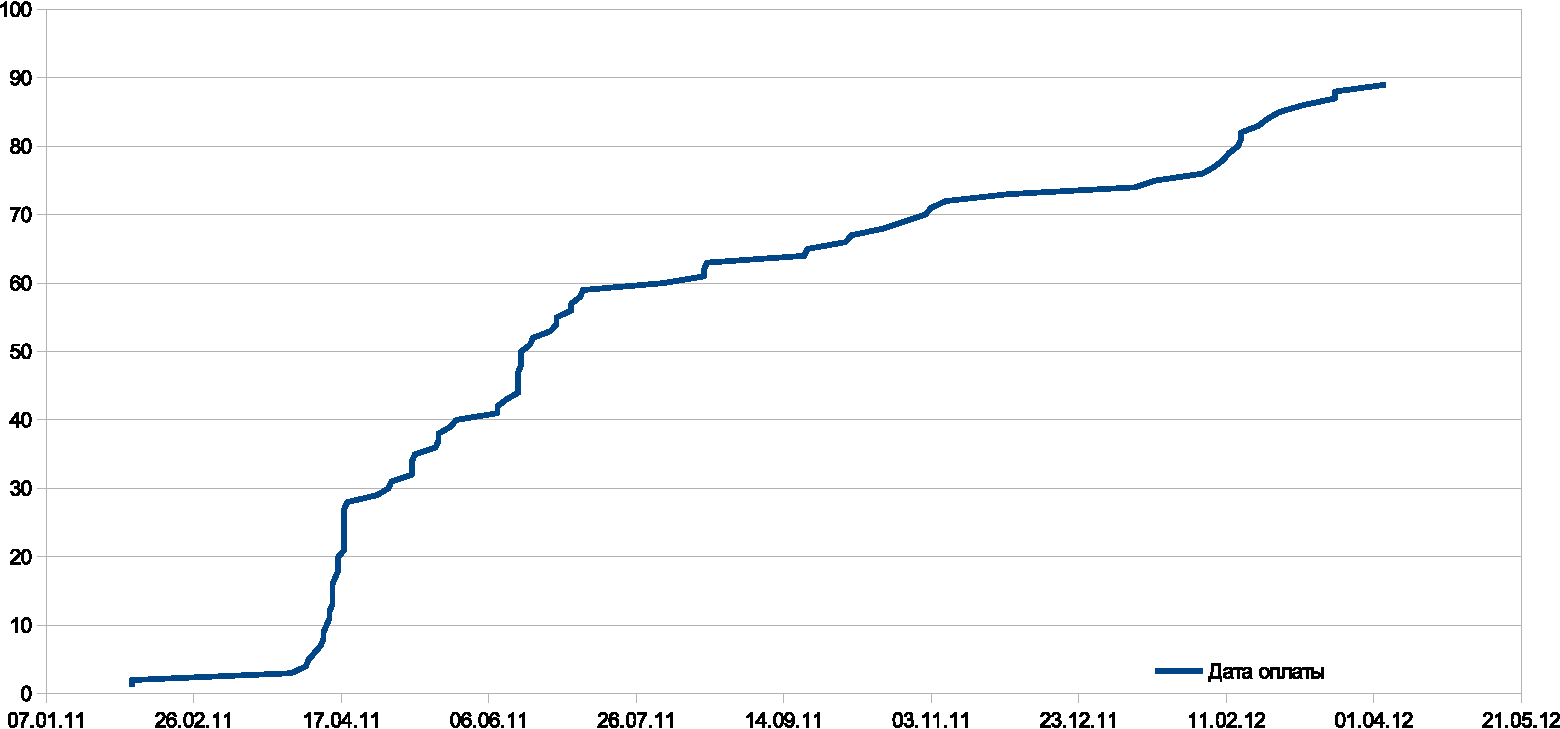
\includegraphics[width=1\textwidth]{members-joining}
\caption{Динамика вступления в МВО}
\end{figure}


Благодаря низкому вступительному взносу и яркой презентации МВО на
<<Открытии сезона-2011>>, весной 2011 года к нам присоединилось
достаточно большое количество человек. Однако, далее темп снизился,
и были месяцы, когда не приходило практически ни одного нового человека.
Во многом это обусловлено невнятной членской программой и, вероятно,
отсутствием заметной снаружи деятельности.


\subsection{Членская программа}

С самого начала был введён членский билет в виде пластиковой карточки,
стилизованный под водительские права. Это было сделано, в том числе,
с расчётом на будущие бонусные программы, возможно с участием партнёров:
скидки в магазинах, кафе, велопрокатах, льготное обслуживание в мастерских
и т.д. Однако такая программа так и не была проработана и внедрена.
Люди, желающие вступить в МВО, делали бы это гораздо охотнее, если
бы, кроме защиты интересов, членство давало пусть небольшие, но бонусы
иного характера.

Из-за того, что Правление и сложившийся актив МВО практически не имеют
опыта публичных акций и кампаний, общество практически не организовывало
каких-либо публичных мероприятий, которые демонстрировали бы наши
достижения и позволяли вербовать новых членов. Деятельность в настоящий
момент проходит в форме переписки или личных контактов с различными
людьми и организациями, при этом её результаты не всегда заметны в
краткосрочном периоде, что также не способствует привлечению новых
людей.


\section{Связи с общественностью}


\subsection{Сайт}

Вначале сайт МВО создавался как визитка организации с площадкой обсуждения
(форумы), а также с целью технической реализации процессов вступления
и членства. С ходом времени на сайте был добавлен раздел <<Документы>>
для публикации официальной переписки объединения, переписки его членов,
стандартов, других документов. Также получила развитие лента новостей,
в которой публикуются в основном собственные материалы, касающиеся
деятельности ОО и велотранспортной тематики. С осени 2011 года в МВО
появился журналист, с целью сделать новости более регулярными и качественными.
На данный момент эта роль является волонтёрской, из-за чего несколько
страдает оперативность. Лента новостей МВО мониторится некоторыми
СМИ, интересующимися велосипедной тематикой, что можно рассматривать
как наше достижение.

Больное место сайта --- дизайн. Среди волонтёров найти дизайнера не
удалось, а на оплату услуг профессионала пока нет средств. Первоначально
дизайн был сделан силами веб-программистов. Встречалось большое количество
отзывов на тему плохого дизайна, в первую очередь <<шапки>>, а также
нестыковок и недоработок как в функциональной части, так и в содержательной
(плохой перевод или его отсутствие, неработоспособность каких-то компонентов,
неудобство использования форума и др.).

В конце 2011 года был произведён небольшой редизайн, лента новостей
была помещена на главную страницу, произведены другие небольшие улучшения.

Изначально сайт был задуман как площадка, открытая для добавления
контента (сообщений, комментариев) лишь членам МВО. На протяжении
года несколько раз поднимался вопрос о том, не стоит ли разрешить
свободный доступ всем желающим для оживления сайта и стимулирования
дискуссий, однако пока всё осталось по-прежнему, в основном по техническим
причинам (проблемы модерации, спама, <<набегов>> идейных противников
и др.).

В ближайшем будущем планируется небольшая реструктуризация сайта (разделы,
выделение страниц/разделов на информацию о проектах, чёткая структура
информации для членов ОО: взносы, членская программа и т.д.).

Вопрос дизайна остаётся открытым.


\subsection{СМИ}

Заметный интерес СМИ к нашему объединению показал, что, действительно,
до сих пор не было достаточно авторитетного и заметного источника
информации на велотранспортную тематику. Налажено постоянное сотрудничество
с сайтами <<Авто-Онлайнер>>, TUT.BY. Выходили различные материалы
в других СМИ, несколько раз представители МВО принимали участие в
записи теле- и радио-передач, в прямых эфирах <<Радио-Минск>>, <<TUT.BY-TV>>.

Как уже говорилось, лента новостей МВО регулярно читается журналистами,
в некоторых случаях новость, опубликованная на нашем сайте, распространяется
по байнету уже в течение нескольких часов после публикации.

К сожалению, на данный момент в организации отсутствует пресс-секретарь
или какой-либо специалист по связям с общественностью, что заметно
ухудшает качество взаимодействия со СМИ.


\section{Деятельность}


\subsection{Акции}


\subsubsection{Праздник <<Открытие сезона-2011>>.}

Мероприятие организовывалось сообществом <<Поехали!>>. Представители
МВО приняли участие в организации праздника в роли волонтёров. Во
время самого мероприятия МВО организовало бесплатный техосмотр велосипедов
для всех желающих, наши самовар и добровольные механики пользовались
большим спросом.

\begin{figure}[ht]
\centering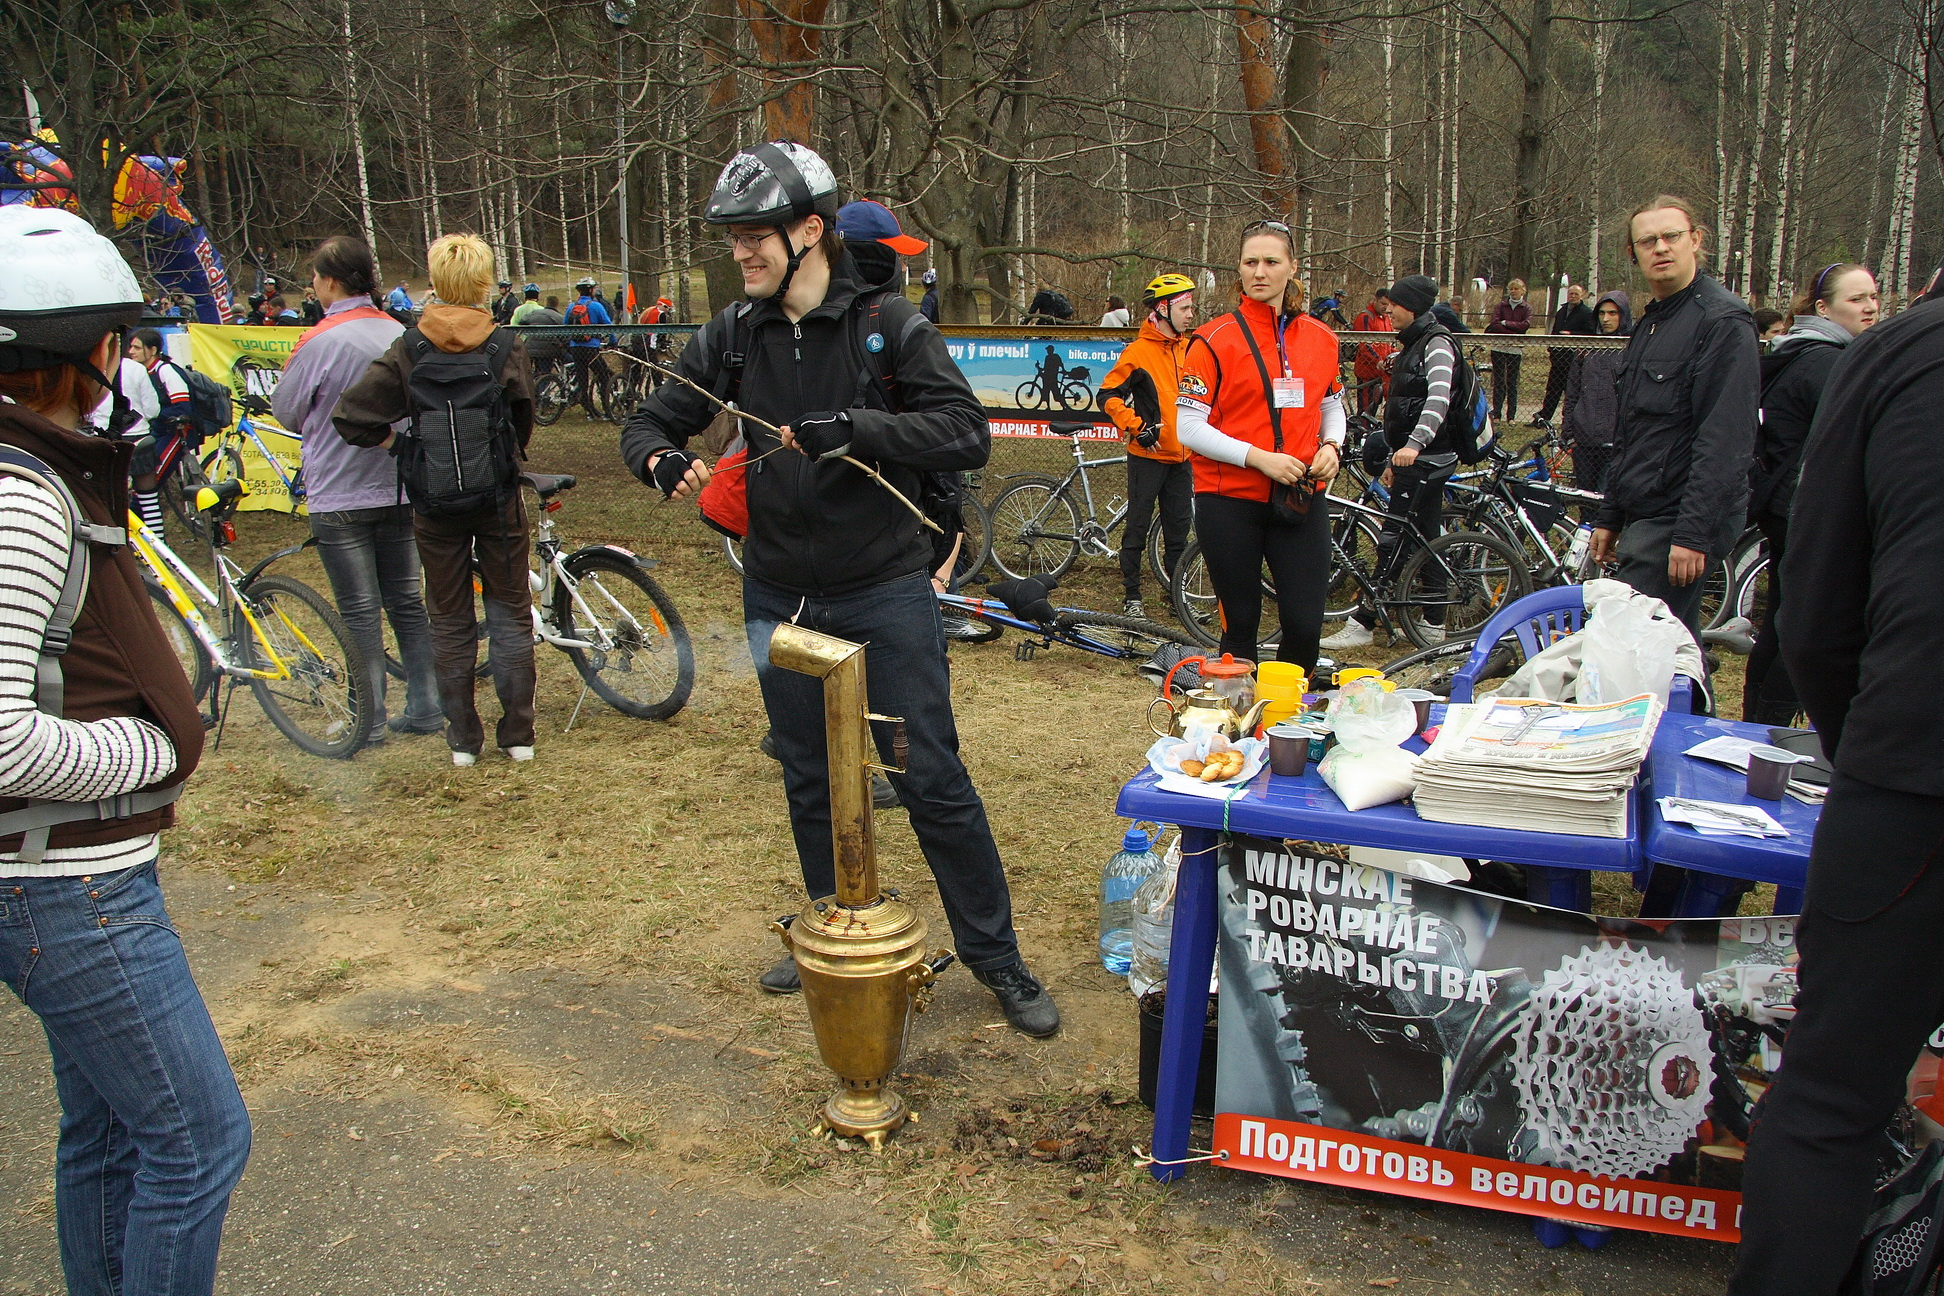
\includegraphics[width=1\textwidth]{bikeopen-2012}\caption{Открытие сезона-2011}
\end{figure}%



\subsubsection{Еженедельные встречи.}

Неформальные встречи МВО начали проводиться с мая 2011 года и, практически
без перерывов, проходят и по сей день. В тёплый сезон мы собирались
в парке Горького, в холодный --- в офисе. Эти встречи, кроме приятного
времяпрепровождения и общения, позволили собрать более-менее постоянный
актив.

\begin{figure}[ht]
\centering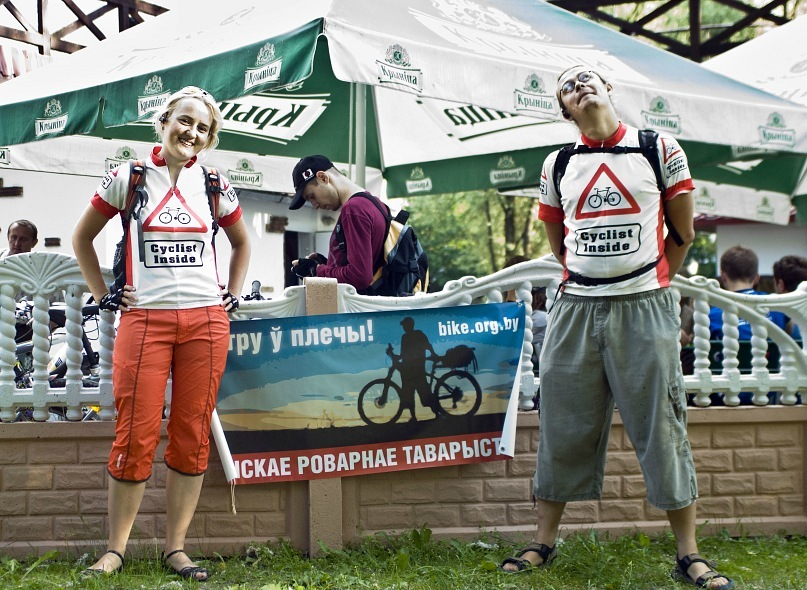
\includegraphics[width=1\textwidth]{weekly-meeting}\caption{Встречи в парке}
\end{figure}%



\subsubsection{Акция <<Сделаем велодорожку безопаснее>>.}

Акция проходила в июне 2011 года, велосипедисты оклеивали световозвращающими
наклейками опасные ограждения велосипедной дорожки вдоль Свислочи. В целом результат достигнут, наклейки держатся. К
сожалению, имели место некоторые недочёты в организации акции (связанные с неожиданно большим количеством участников) и её освещении в СМИ.

\begin{figure}[ht]
\centering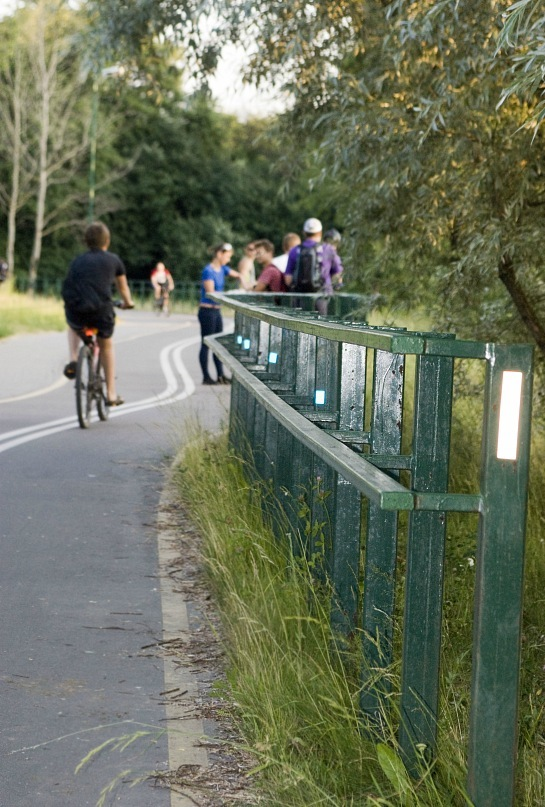
\includegraphics[height=0.3\textheight]{y_b19e375b}

\caption{<<Сделаем велодорожку безопаснее>>}
\end{figure}%



\subsubsection{Участие в Велофоруме-2011, Киев.}

Украинский "Велофорум" --- ежегодная конференция, посвящённая проблеме городского велосипедного транспорта. Проходит
каждый раз в новом городе. В 2011 году её принимал Киев, и от МВО участвовали два человека: Евгений Хоружий и Ольга
Карабутова. Там мы познакомились с руководством Европейской федерации велосипедистов, с коллегами из украинских городов.
Удивила представительность конференции: присутствовали люди из администраций нескольких городов, и даже лично мэр города
Долина.

\begin{figure}[ht]
\centering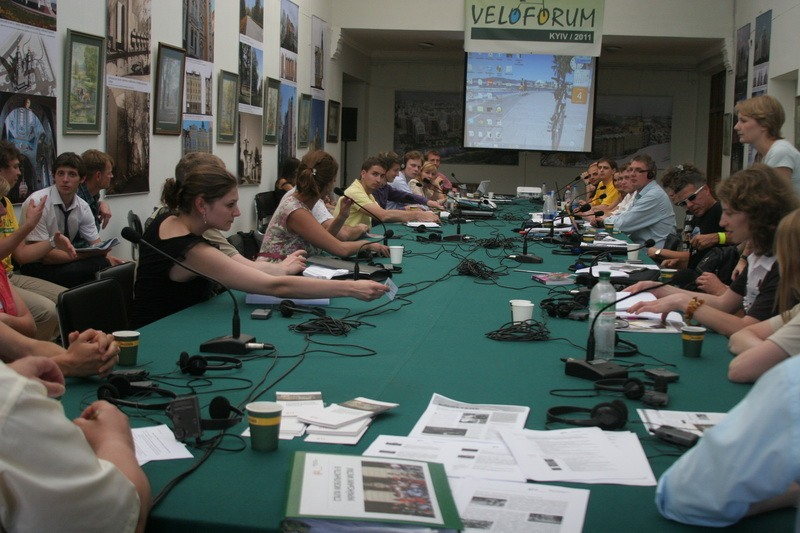
\includegraphics[width=1\textwidth]{veloforum}

\caption{Велофорум, Киев}
\end{figure}%



\subsubsection{Участие в первом белорусском Велофоруме, Гродно.}

Наши коллеги из Гродно в сентябре 2011 года собрали наш, белорусский, велофорум для координации наших усилий по развитию
велосипедного движения. Там мы познакомились друг с другом, поделились опытом, нагенерировали целую кучу идей.


\subsubsection{Вступление в <<Зелёную сеть>>.}
<<Зелёная сеть>> --- экологическое товарищество, объединяющее белорусские экологические организации. Несмотря на то, что
МВО не является экологической организацией в чистом виде, тема велосипедного транспорта очень тесно переплетается с
темами экологии и устойчивого развития городов. Членство в <<Зелёной сети>> позволило нам наладить контакты с
NGO-сообществом Беларуси, познакомиться с опытом коллег, получить информационную поддержку.


\subsubsection{Участие в пилотном проекте <<Велодорожка по проспекту Независимости>>.}

В рамках <<Концепции обеспечения велосипедного движения в г.~Минске>> в 2011~г. реализовывался пилотный проект по
обустройству велосипедной дорожки по главному проспекту столицы. МВО принимало участие в этом на уровне представления
требований велосипедистов к такой дорожке, участвовало в обсуждениях технических решений, проводило обследования
местности.

\subsubsection{Безбарьерная среда.}

В 2011 году мы проводили так называемую <<разведку боем>>, чтобы узнать, в чём же причина столь вопиющего несоблюдения
строительных норм, касающихся создания безбарьерной среды: писали обращения в администрации районов, Госстройнадзор,
проектные организации по конкретным объектам с просьбами исправить нарушения. Как показала практика, такие обращения
имеют невысокую эффективность из-за непонимания чиновниками сути проблемы и формального отношения к ней.

Однако, такая разведка позволила собрать необходимую информацию. Так, были получены подтверждения тому, что нарушения
норм имеют место ещё на этапах проектирования, а отсутствие должного контроля при экспертизе, строительстве, приёмке
объектов лишь усугубляют ситуацию.


\subsubsection{Проект TANDEM.}

В конце 2011 года мы выиграли мини-грант проекта TANDEM. Проект, который будет осуществляться, направлен на улучшение
велосипедной инфраструктуры в одном из микрорайонов города Минска. В рамках него мы, совместно с жителями, попробуем
создать место для хранения велосипедов, оборудовать образцовую велопарковку, подготовить предложения по обустройству
внутримикрорайонных велосипедных путей. Также в рамках проекта будет поднята дискуссия о проблемах безбарьерной среды, о
проектировании велосипедной инфраструктуры. Будут созданы технические рекомендации по обустройству парковок и мест
хранения, организации велодорожек.


\subsubsection{Карта препятствий.}

Весной появился сайт {\tt kerbs.bike.org.by} --- карта, на которой каждый может обозначить существующие препятствия для
велосипедистов. В течение первого же месяца работы этого сайта количество объектов достигло примерно трёх тысяч, а
визуально весь Минск представлен как одно большое препятствие. Практического применения карта пока не нашла, но как
инструмент демонстрации того, насколько существующее положение вещей печально, она отлично годится.

\subsubsection{Защита интересов велосипедистов.}

В 2011 году к нам обратился лишь один член МВО за помощью в отстаивании своих прав. Владимир Володин пытался через суд
доказать, что в месте, где его оштрафовали инспекторы ГАИ за проезд по проезжей части, движение по тротуару было
невозможным, а, значит, нарушения ПДД не было. МВО помогло с консультацией адвоката, однако суд с доводами не
согласился.


\section{Финансирование}

Бюджет МВО в 2011 году складывался из добровольных пожертвований физлиц и членских взносов. В приложении приводится отчёт о
целевом использовании полученных средств.

Основные затраты пришлись на этап отсутствия бухгалтера, когда МВО было вынуждено платить за ведение
бухгалтерии сторонней организации. С середины лета у нас появился свой бухгалтер-волонтёр, и данная проблема
разрешилась.

\appendix

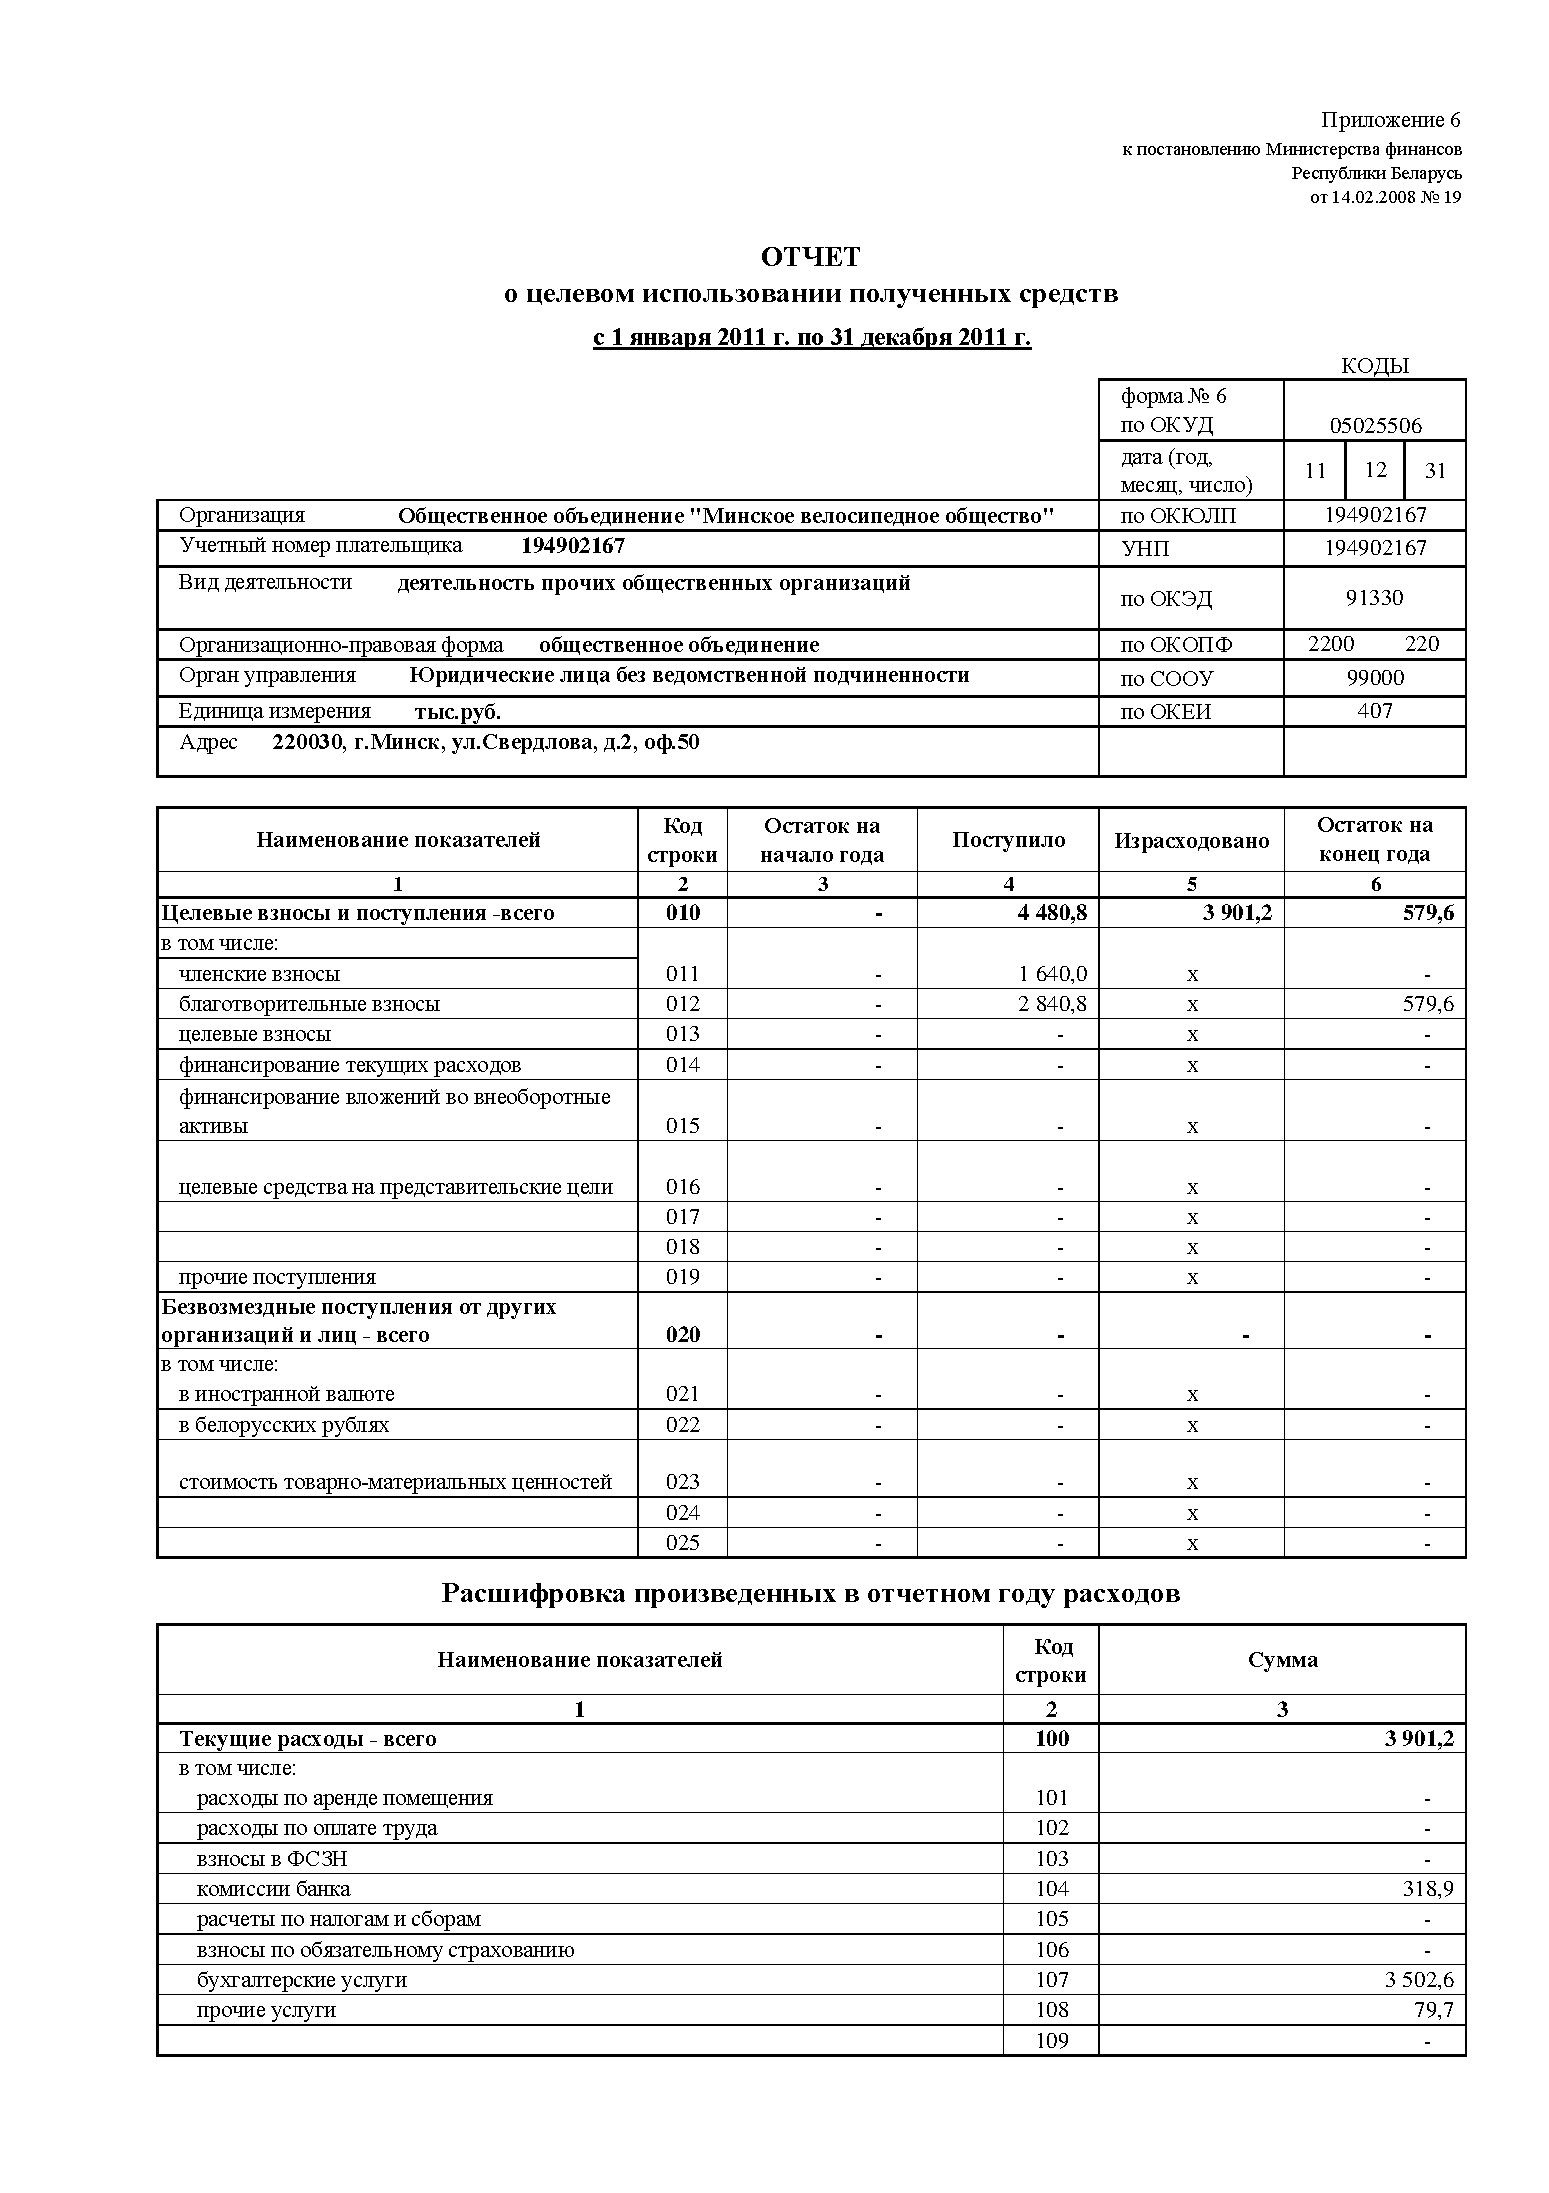
\includepdf[pages=-]{balans-2011-target.pdf}

\end{document}
